%% ============================================================
%%  BORRADOR — La Gaceta de la Real Sociedad Matemática Española
%%  Adaptar al fichero de clase oficial de la revista antes del envío
%% ============================================================
\documentclass[11pt,a4paper]{article}

% --- Codificación y lengua ---
\usepackage[utf8]{inputenc}
\usepackage[T1]{fontenc}
\usepackage{lmodern}
% babel spanish not available in this TeX installation
\usepackage{microtype}

% --- Matemáticas ---
\usepackage{amsmath,amsthm,amssymb,amsfonts}
\usepackage{mathtools}

% --- Geometría ---
\usepackage[top=2.5cm,bottom=2.5cm,left=3cm,right=3cm]{geometry}

% --- Gráficos ---
\usepackage{graphicx}
\usepackage{xcolor}
\usepackage{float}
\usepackage{caption}
\usepackage{subcaption}

% --- Código ---
\usepackage{listings}
\lstset{
  basicstyle      = \small\ttfamily,
  keywordstyle    = \color{blue!70!black}\bfseries,
  commentstyle    = \color{green!50!black}\itshape,
  stringstyle     = \color{orange!80!black},
  backgroundcolor = \color{gray!8},
  frame           = single,
  framerule       = 0.4pt,
  rulecolor       = \color{gray!40},
  breaklines      = true,
  columns         = flexible,
  numbers         = none,
  xleftmargin     = 6pt,
  xrightmargin    = 6pt,
}

% --- Tablas ---
\usepackage{booktabs}
\usepackage{array}

% --- Hipervínculos ---
\usepackage[colorlinks=true,
            linkcolor=blue!60!black,
            citecolor=green!40!black,
            urlcolor=blue!70!black]{hyperref}

% --- Entornos matemáticos ---
\theoremstyle{plain}
\newtheorem{teorema}{Teorema}[section]
\newtheorem{proposicion}[teorema]{Proposición}
\newtheorem{corolario}[teorema]{Corolario}
\newtheorem{lema}[teorema]{Lema}

\theoremstyle{definition}
\newtheorem{definicion}[teorema]{Definición}
\newtheorem{ejemplo}[teorema]{Ejemplo}

\theoremstyle{remark}
\newtheorem{observacion}[teorema]{Observación}

% --- Macros ---
\newcommand{\C}{\mathbb{C}}
\newcommand{\R}{\mathbb{R}}
\newcommand{\N}{\mathbb{N}}
\newcommand{\Puno}{\mathbb{P}^1(\mathbb{C})}
\newcommand{\fn}[1]{\texttt{#1}}
\newcommand{\pkg}[1]{\textsl{#1}}
\DeclareMathOperator{\grad}{grado}

% --- Datos del artículo ---
\title{\textbf{Dinámica de funciones racionales en la esfera de Riemann:
       geometría, cuencas de atracción y visualización}}

\author{Luis Javier Hernández Paricio\\
        {\small Departamento de Matemáticas y Computación}\\
        {\small Universidad de La Rioja, Logroño}\\
        {\small \texttt{luis-javier.hernandez@unirioja.es}}}

\date{} % La fecha la pone la revista

% ============================================================
\begin{document}
% ============================================================

\maketitle

\begin{abstract}
Estudiamos la dinámica de iteración de funciones racionales desde la
perspectiva natural de la esfera de Riemann~$\Puno$.
El uso de coordenadas homogéneas elimina el carácter especial del punto
en el infinito y permite ver la dinámica completa: cuencas de atracción
que envuelven la esfera, fronteras fractales que conectan todas las
cartas, y puntos fijos en el infinito que quedan ocultos cuando se
trabaja únicamente en~$\C$.
Ilustramos la teoría con los ejemplos clásicos de Milnor —Newton,
Halley, la familia $z^2+c$— e incluimos la visualización de cuencas
de ciclos periódicos de período~$p\geq 2$, implementada en el paquete
\pkg{RiemannBasins.jl} que acompaña al artículo.
Una parte significativa del trabajo está dedicada al diseño de
visualizaciones inclusivas: describimos criterios matemáticamente
fundados basados en el espacio de color perceptualmente uniforme LCHab
y en la paleta Okabe--Ito, que garantiza que las figuras sean
igualmente legibles para personas con daltonismo.
El código es de libre acceso y reproducible.
\end{abstract}

\bigskip
\noindent\textbf{Palabras clave:} esfera de Riemann, coordenadas homogéneas,
cuencas de atracción, ciclos periódicos, conjunto de Julia, método de Newton,
espacio de color LCHab, visualización inclusiva, daltonismo.

\medskip
\noindent\textbf{MSC 2020:} 37F10, 37F45, 32H50, 68U05.

% ============================================================
\section{Introducción}
% ============================================================

El método de Newton aplicado al polinomio $P(z)=z^3-1$ produce, a partir
de cualquier punto inicial $z_0\in\C$, la sucesión de iterados
\[
   z_{n+1} = z_n - \frac{P(z_n)}{P'(z_n)}
           = \frac{2z_n^3+1}{3z_n^2},
\]
que converge a una de las tres raíces cúbicas de la unidad,
$1,\,\omega=e^{2\pi i/3},\,\omega^2=e^{4\pi i/3}$, según la posición de
$z_0$.
Colorear cada punto $z_0$ según la raíz a la que converge su órbita
produce la figura~\ref{fig:newton_z3}: un fractal con simetría de orden
tres en el que las tres cuencas de atracción se entrelazan de forma
infinitamente intrincada en su frontera común.

\begin{figure}[ht]
  \centering
  % Comando: basin_portrait([1,0,0,-1],[0,3,0,0]; bands=8.0)
  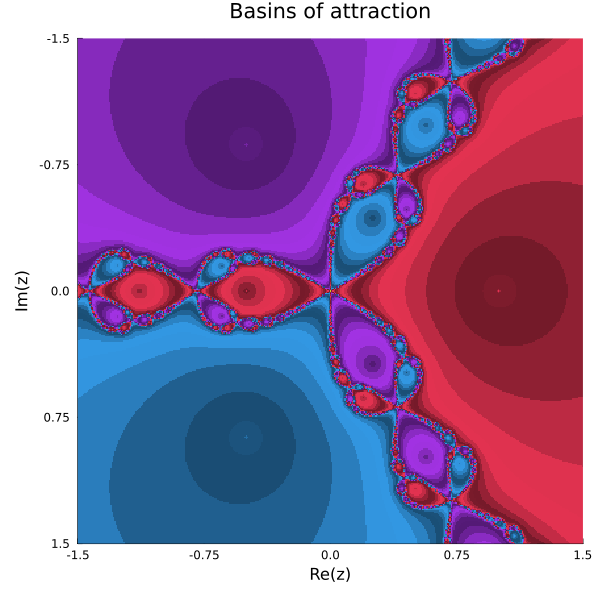
\includegraphics[width=0.55\textwidth]{figures/newton_z3_test.png}
  \caption{Cuencas de atracción del método de Newton para $z^3-1$,
           generadas con la paleta LCHab de \pkg{RiemannBasins.jl}.
           Cada punto se colorea según la raíz a la que converge su
           órbita; los tres tonos tienen luminosidad CIE~$L^*$ idéntica,
           por lo que ninguna cuenca destaca sobre las demás.
           Las bandas concéntricas revelan la velocidad de convergencia
           mediante modulación del canal de luminosidad.}
  \label{fig:newton_z3}
\end{figure}

Esta imagen suscita una pregunta inmediata: ¿qué ocurre con los puntos
que «escapan hacia el infinito»?
En el plano complejo, $\infty$ es una singularidad que se trata de forma
ad hoc.
Sin embargo, para la función racional $f(z)=(2z^3+1)/(3z^2)$, el punto
$\infty$ es también un punto fijo —de hecho, repulsor— con un papel
perfectamente bien definido en la dinámica global.
Verlo requiere salir de~$\C$ y trabajar en su compactificación natural:
la \emph{esfera de Riemann}~$\Puno$.

El presente artículo tiene cuatro objetivos.
El primero es mostrar que $\Puno$, lejos de ser una complicación
abstracta, es el marco más sencillo para estudiar la dinámica de
funciones racionales: elimina los casos especiales ligados al infinito y
hace manifiesta la simetría global de los sistemas.
El segundo es ilustrar la teoría con los ejemplos más iluminadores de la
literatura, en particular los del libro seminal de Milnor~\cite{Milnor2006},
y extenderlos a la visualización de cuencas de ciclos periódicos de
período~$p\geq 2$.
El tercero es describir cómo diseñar visualizaciones matemáticamente
coherentes de las cuencas, usando el espacio de color LCHab para
garantizar que todos los tonos sean perceptualmente equivalentes.
El cuarto —y quizá el menos habitual en la literatura matemática— es
el compromiso con la \emph{inclusión visual}: todas las figuras del
artículo están disponibles también en una paleta accesible para personas
con daltonismo (deuteranopía y protanopía), siguiendo las directrices
de Okabe e~Ito~\cite{OkabeIto2008}.
Con ello, el artículo se suma a la creciente demanda de comunicación
científica accesible para toda la audiencia.

% ============================================================
\section{La esfera de Riemann}
\label{sec:esfera}
% ============================================================

\subsection{Proyección estereográfica}

La \emph{esfera unidad} $S^2\subset\R^3$ es el conjunto de puntos
$(x,y,t)$ con $x^2+y^2+t^2=1$.
La \emph{proyección estereográfica} desde el polo norte $N=(0,0,1)$
identifica cada punto $(x,y,t)\in S^2\setminus\{N\}$ con el número
complejo
\[
  z = \frac{x+iy}{1-t}\;\in\;\C,
\]
y extiende la biyección al plano añadido $N\leftrightarrow\infty$,
obteniendo así la \emph{esfera de Riemann} $\hat{\C}=\C\cup\{\infty\}$.
La fórmula inversa es
\[
   (x,y,t) = \left(\frac{2\operatorname{Re}(z)}{|z|^2+1},\;
                    \frac{2\operatorname{Im}(z)}{|z|^2+1},\;
                    \frac{|z|^2-1}{|z|^2+1}\right).
\]

\begin{observacion}
La proyección estereográfica es conforme (preserva ángulos) pero no
isométrica.
Los círculos y rectas del plano corresponden exactamente a los
círculos en~$S^2$, propiedad fundamental en la teoría de las
transformaciones de Möbius.
\end{observacion}

\subsection{El espacio proyectivo \texorpdfstring{$\Puno$}{P1(C)}}

Existe otra realización de la esfera de Riemann, algebraicamente más
limpia, que resulta esencial cuando se trabaja con funciones racionales:
el \emph{espacio proyectivo complejo unidimensional}~$\Puno$.

Se define como el cociente
\[
  \Puno = \bigl(\C^2\setminus\{(0,0)\}\bigr)\,\big/\!\sim,
\]
donde $(z_0,z_1)\sim(\lambda z_0,\lambda z_1)$ para todo
$\lambda\in\C^*$.
La clase de equivalencia de $(z_0,z_1)$ se escribe $[z_0:z_1]$ y se
llama \emph{punto homogéneo}.

El espacio $\Puno$ se cubre con dos cartas afines:
\begin{align*}
  U_0 &= \{[z_0:z_1]\;:\;z_1\neq 0\},
  &z &= z_0/z_1\;\in\;\C,\\
  U_1 &= \{[z_0:z_1]\;:\;z_0\neq 0\},
  &w &= z_1/z_0\;\in\;\C.
\end{align*}
En la intersección $U_0\cap U_1$, el cambio de carta es $w=1/z$, de modo
que el punto $[1:0]\in U_1$ (con $w=0$) corresponde al punto en el
infinito de la carta~$U_0$.
Así, $\Puno\cong\hat{\C}$ como superficies de Riemann.

La ventaja de $\Puno$ sobre~$\hat{\C}$ es simétrica: ningún punto
ocupa un lugar especial.
Trabajar en coordenadas homogéneas $[z_0:z_1]$ evita los casos
separados «$z$ finito» frente a «$z=\infty$».

% ============================================================
\section{Funciones racionales en \texorpdfstring{$\Puno$}{P1(C)}}
\label{sec:racionales}
% ============================================================

\subsection{Extensión natural al espacio proyectivo}

Una \emph{función racional} $f:\C\to\hat{\C}$ se escribe
$f(z)=p(z)/q(z)$ con $p,q$ polinomios sin factor común.
Su \emph{grado} es $d=\max(\deg p,\deg q)$.
Para extenderla a $\Puno$ de forma regular —incluyendo el punto en el
infinito— se homogenizan el numerador y el denominador:
\[
  P(z_0,z_1) = z_1^d\,p\!\left(\tfrac{z_0}{z_1}\right),\qquad
  Q(z_0,z_1) = z_1^d\,q\!\left(\tfrac{z_0}{z_1}\right).
\]
Ambos son polinomios homogéneos de grado~$d$, y la aplicación
\[
  F:\Puno\longrightarrow\Puno,\qquad
  [z_0:z_1]\longmapsto [P(z_0,z_1):Q(z_0,z_1)]
\]
está bien definida (el cociente $[P:\!Q]$ no depende del representante)
y es holomorfa.
En la carta afín $z=z_0/z_1$ recuperamos $f(z)=p(z)/q(z)$; en la carta
$w=z_1/z_0$ la función toma la forma regular $\tilde{f}(w)$ sin polos.

\begin{ejemplo}[Newton para $z^3-1$]
$f(z)=(2z^3+1)/(3z^2)$, de grado~$3$.
Homogeneizando con $d=3$:
$P(z_0,z_1)=2z_0^3+z_1^3$,\; $Q(z_0,z_1)=3z_0^2 z_1$.
En la carta $w$:
\[
   \tilde{f}(w) = \frac{3w}{2+w^3},\qquad\tilde{f}(0)=0,\qquad
   \tilde{f}'(0)=\tfrac{3}{2}.
\]
El punto $[1:0]$ (infinito en la carta $z$) tiene imagen $[1:0]$ y
multiplicador~$3/2>1$: es un \emph{punto fijo repulsor}.
\end{ejemplo}

\subsection{Puntos fijos y su multiplicador}

Un \emph{punto fijo} de $f$ en $\Puno$ es un punto $\zeta$ con
$f(\zeta)=\zeta$.
Para un punto fijo finito $\zeta\in\C$, el \emph{multiplicador} es
$\lambda=f'(\zeta)\in\C$.
Para el punto $\zeta=\infty$, se usa la carta $w=1/z$: el multiplicador
es la derivada de $\tilde{f}$ en $w=0$.

La clasificación por el módulo del multiplicador es la habitual:
\begin{itemize}
  \item $|\lambda|<1$: punto fijo \emph{atractor} (superatractor si $\lambda=0$).
  \item $|\lambda|=1$: punto fijo \emph{indiferente}.
  \item $|\lambda|>1$: punto fijo \emph{repulsor}.
\end{itemize}

El siguiente resultado es uno de los más elegantes de la teoría:

\begin{teorema}[Conteo de puntos fijos en $\Puno$]
\label{teo:puntosfijos}
Una función racional de grado $d\geq 1$ tiene exactamente $d+1$
puntos fijos en~$\Puno$, contados con multiplicidad.
\end{teorema}

\begin{proof}[Demostración (esquema)]
Los puntos fijos son las soluciones de $F([z_0:z_1])=[z_0:z_1]$,
es decir, $[P(z_0,z_1):Q(z_0,z_1)]=[z_0:z_1]$.
Esto equivale a $z_1 P(z_0,z_1)-z_0 Q(z_0,z_1)=0$, un polinomio
homogéneo de grado $d+1$, que por el teorema de Bézout proyectivo
tiene exactamente $d+1$ raíces (con multiplicidad) en~$\Puno$.
\end{proof}

Para el método de Newton de un polinomio $P$ de grado $n$, la función
$f$ tiene grado $n$, sus $n$ puntos fijos finitos son exactamente
las raíces de~$P$ (todas superatractoras, pues $f'(\zeta)=0$ en toda
raíz simple), y el punto en el infinito es el $n+1$-ésimo punto fijo.

% ============================================================
\section{Cuencas de atracción y conjuntos de Julia}
\label{sec:cuencas}
% ============================================================

\subsection{Conjuntos de Fatou y de Julia}

Dada una función racional $f:\Puno\to\Puno$ de grado $d\geq 2$,
definimos el \emph{conjunto de Fatou} $\mathcal{F}(f)$ como el mayor
abierto de $\Puno$ en el que la familia de iterados
$\{f^n\}_{n\geq 1}$ es una familia normal (en el sentido de Montel).
Su complementario $\mathcal{J}(f)=\Puno\setminus\mathcal{F}(f)$ es el
\emph{conjunto de Julia}.

Intuitivamente, $\mathcal{F}(f)$ es la región de dinámica estable
—pequeñas perturbaciones del punto inicial producen pequeñas
perturbaciones de la órbita—, mientras que $\mathcal{J}(f)$ es la
región de dinámica caótica, donde la sensibilidad a las condiciones
iniciales es máxima.

\begin{proposicion}[Propiedades del conjunto de Julia]
$\mathcal{J}(f)$ es compacto, no vacío, perfectamente invariante
($f^{-1}(\mathcal{J})=\mathcal{J}=f(\mathcal{J})$), y es la
adherencia del conjunto de puntos periódicos repulsores.
\end{proposicion}

\subsection{Cuencas de atracción}

La \emph{cuenca de atracción inmediata} de un punto fijo atractor
$\zeta$ es
\[
  \mathcal{A}^*(\zeta)=\{z\in\Puno\;:\;f^n(z)\to\zeta,\;
  f^n(z)\text{ permanece cerca de }\zeta\}.
\]
La \emph{cuenca de atracción total} $\mathcal{A}(\zeta)$ incluye
además todas las preimágenes iteradas de $\mathcal{A}^*(\zeta)$.
Un resultado fundamental de Fatou garantiza que $\mathcal{A}^*(\zeta)$
es simplemente conexo si el punto crítico de $f$ más cercano cae en~$\mathcal{A}^*(\zeta)$.

La frontera de cada cuenca de atracción es precisamente el conjunto
de Julia $\mathcal{J}(f)$.
En los ejemplos del método de Newton, $\mathcal{J}(f)$ separa las
cuencas de las distintas raíces: su geometría fractal —habitualmente
de dimensión de Hausdorff estrictamente entre 1 y 2— es la que produce
las imágenes más llamativas.

\subsection{Clasificación de los componentes de Fatou}

El teorema de clasificación de Fatou y Sullivan establece que todo
componente periódico del conjunto de Fatou es de uno de estos cinco
tipos:

\begin{enumerate}
  \item \textbf{Cuenca de atractor fijo:} $f^n(z)\to\zeta$ con $|\lambda|<1$.
  \item \textbf{Cuenca de ciclo atractor:} $f^{np}(z)\to\zeta_j$ donde
        $\{\zeta_1,\ldots,\zeta_p\}$ es un ciclo de período $p\geq 2$.
  \item \textbf{Cuenca parabólica:} convergencia a un punto fijo de
        multiplicador $\lambda=e^{2\pi i r}$, $r\in\mathbb{Q}$.
  \item \textbf{Disco de Siegel:} componente simplemente conexo con
        dinámica de rotación irracional.
  \item \textbf{Anillo de Herman:} componente doblemente conexo (topología de corona)
        con dinámica de rotación irracional.
\end{enumerate}

Para el método de Newton de un polinomio, solo aparecen cuencas del
tipo~(i) —las raíces son superatractoras— y eventualmente del tipo~(iii)
para polinomios con raíces múltiples.
Los tipos~(iv) y~(v) requieren funciones racionales con propiedades
aritméticas muy especiales en los multiplicadores.

% ============================================================
\section{Ejemplos clásicos}
\label{sec:ejemplos}
% ============================================================

\subsection{Newton para \texorpdfstring{$z^3-1$}{z3-1}: el ejemplo fundamental}

Como ya vimos, $f(z)=(2z^3+1)/(3z^2)$ tiene grado 3 y cuatro puntos
fijos en~$\Puno$: las tres raíces cúbicas de la unidad (superatractoras)
y el infinito (repulsor con multiplicador~$3/2$).

Por el Teorema~\ref{teo:puntosfijos}, $3+1=4$ puntos fijos, y efectivamente
los encontramos todos.
La simetría del sistema bajo la rotación $z\mapsto\omega z$ garantiza
que las tres cuencas tienen exactamente la misma forma, rotadas entre
sí $120^\circ$.

La frontera entre las cuencas —el conjunto de Julia $\mathcal{J}(f)$—
tiene una propiedad sorprendente conocida desde Fatou (1919): \emph{en
todo punto de la frontera de una cuenca se acumulan puntos de las otras
dos cuencas}.
Esto implica que los tres colores aparecen simultáneamente en cualquier
ampliación arbitraria de la frontera.

\begin{figure}[ht]
  \centering
  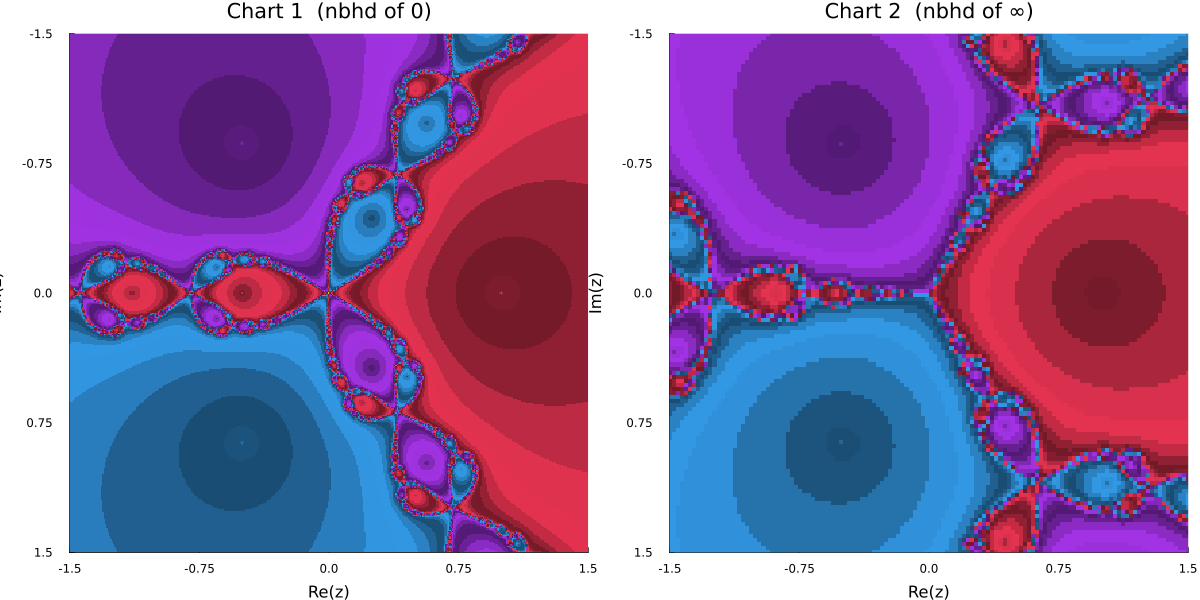
\includegraphics[width=0.90\textwidth]{figures/newton_two_charts.png}
  \caption{Newton para $z^3-1$ en las dos cartas de $\Puno$.
           La carta afín estándar (izquierda) muestra las tres cuencas
           con simetría ternaria.
           La segunda carta estereográfica (derecha) revela que el punto
           en el infinito es repulsor y queda en la frontera de las tres
           cuencas, oculto en la representación plana habitual.
           Generado con \pkg{RiemannBasins.jl}.}
  \label{fig:newton_z3_doble}
\end{figure}

\subsection{Newton para \texorpdfstring{$z^4-1$}{z4-1}: el infinito como cuenca}

Para $P(z)=z^4-1$, el método de Newton da
\[
  f(z)=\frac{3z^4+1}{4z^3},\quad d=4,
\]
con cinco puntos fijos en $\Puno$: las cuatro raíces cuartas de la
unidad ($1,i,-1,-i$, todas superatractoras) y el infinito.

Ahora la imagen de $f$ en la segunda carta $w=1/z$ es
$\tilde{f}(w)=4w/(3+w^4)$,
con $\tilde{f}(0)=0$ y $\tilde{f}'(0)=4/3$.
El punto en el infinito es de nuevo repulsor (multiplicador~$4/3$).

\begin{figure}[ht]
  \centering
  % Comando: two_chart_portrait([1,0,0,0,3],[0,0,0,4,0]; bands=8.0, savepath="figures/newton_z4_two_charts.png")
  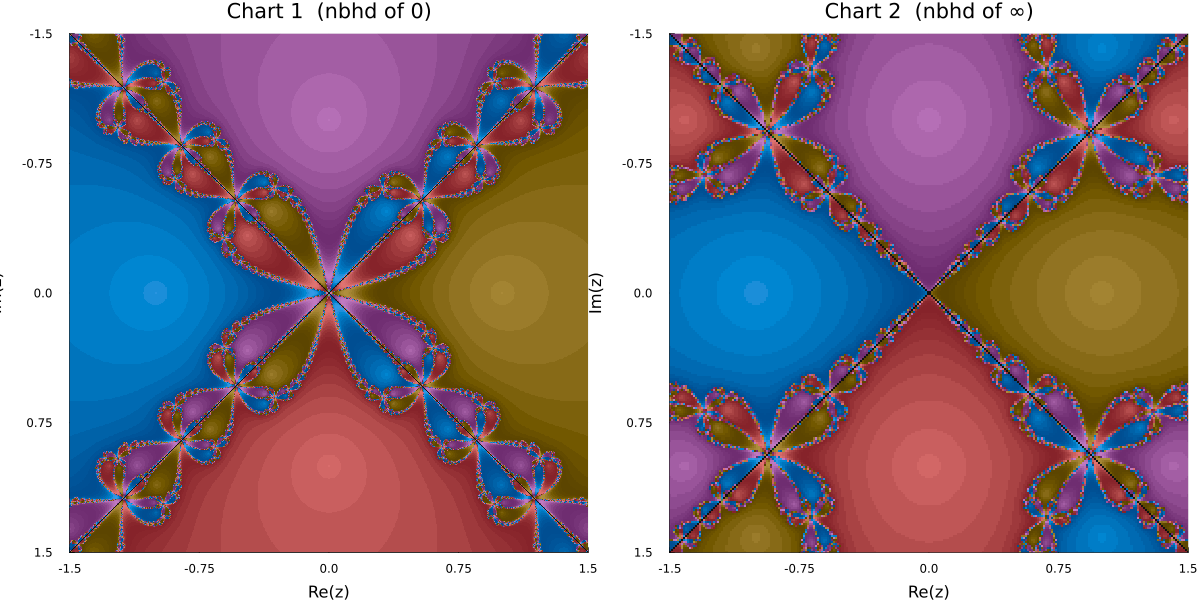
\includegraphics[width=0.90\textwidth]{figures/newton_z4_two_charts.png}
  \caption{Newton para $z^4-1$ en las dos cartas de $\Puno$ (carta~1 a la izquierda, carta~2 a la derecha).
           En la segunda carta se aprecia la cuenca que rodea el punto en
           el infinito (repulsor), oculta en la representaci\'{o}n plana
           habitual.
           Generado con el paquete \pkg{RiemannBasins.jl}.}
  \label{fig:newton_z4}
\end{figure}

La segunda carta revela la estructura global de la dinámica: las cuatro
cuencas se distribuyen simétricamente en torno al repulsor en el
infinito, y la frontera fractal tiene simetría de orden cuatro.
Esta imagen es imposible de obtener si se trabaja únicamente en~$\C$.

\subsection{El método de Halley}

El \emph{método de Halley} para el polinomio $P$ es el esquema de orden
cúbico
\[
   z_{n+1} = z_n - \frac{2P(z_n)P'(z_n)}{2[P'(z_n)]^2-P(z_n)P''(z_n)}.
\]
Aplicado a $P(z)=z^3-1$, produce una función racional de grado~5 cuyos
puntos fijos finitos son también las raíces de~$P$, pero las cuencas
de atracción son más «anchas» y la frontera fractal, aunque sigue siendo
el conjunto de Julia, tiene una geometría diferente a la del método de
Newton.

\begin{figure}[ht]
  \centering
  % Comando: two_chart_portrait(halley_num, halley_den; bands=8.0)
  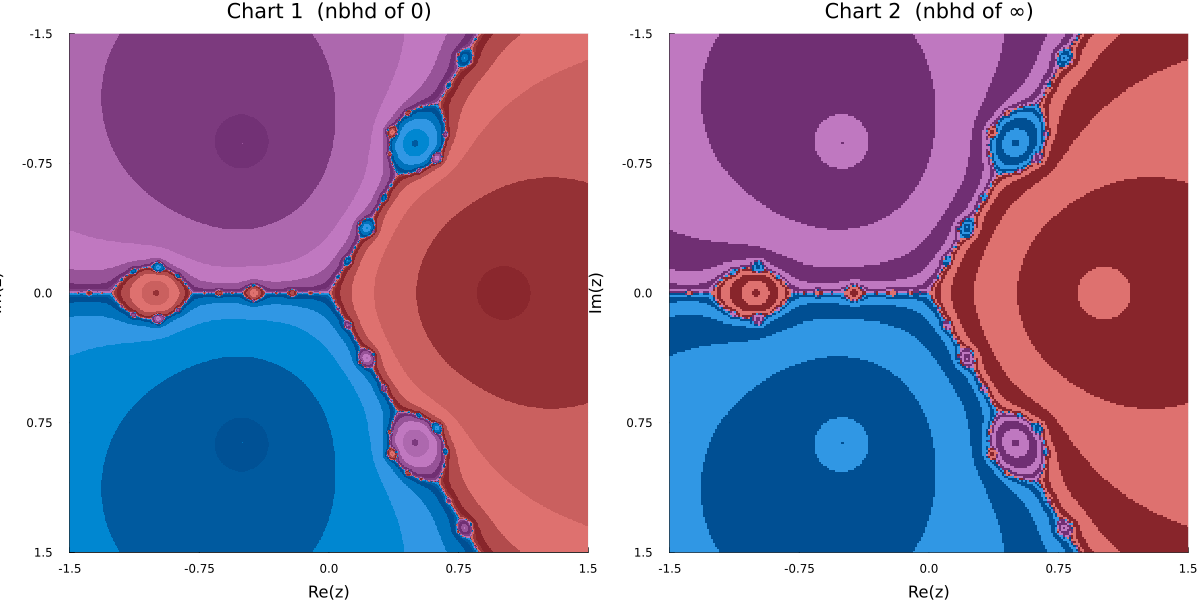
\includegraphics[width=0.75\textwidth]{figures/halley_z3_two_charts.png}
  \caption{Método de Halley para $z^3-1$ en las dos cartas de $\Puno$.
           Las cuencas son más regulares que en Newton y la frontera
           fractal es más suave.}
  \label{fig:halley}
\end{figure}

La comparación entre Newton y Halley ilustra cómo distintos métodos
numéricos para un mismo problema producen estructuras topológicas
globalmente diferentes en~$\Puno$, aunque compartan las mismas
cuencas de atracción finales.

\subsection{Una familia de Milnor: \texorpdfstring{$z^2+c$}{z2+c}}

Las funciones $f_c(z)=z^2+c$ con $c\in\C$ son el ejemplo prototípico
de la teoría de polinomios de Milnor.
Para ciertos valores de~$c$, la órbita del punto crítico $z=0$ converge
a un ciclo atractor de período~$p$, dando lugar a cuencas de una
complejidad topológica creciente.

\begin{itemize}
  \item $c=0$: $f_0(z)=z^2$, cuenca de atracción de $0$ es el disco
        unitario; cuenca de atracción de $\infty$ es el exterior.
  \item $c=-1$: existe un ciclo atractor $\{0,-1\}$ de período~2.
        La cuenca tiene una estructura de «conejo de Douady».
  \item $c=-2$: $f_{-2}$ tiene un punto de Julia real ($[-2,2]$);
        cuencas de $\pm\infty$ son todo el complementario.
\end{itemize}

En todos los casos, $\infty$ es un punto fijo superatractor de la
extensión a $\Puno$: la cuenca del infinito es la componente de Fatou
exterior, que en la segunda carta estereográfica aparece como la cuenca
central del repulsor en~$0$.

\subsection{Cuencas de ciclos periódicos: \texorpdfstring{$z^2-1$}{z2-1}}
\label{ssec:pcycle_z2}

La función $f(z)=z^2-1$ es el caso $c=-1$ de la familia de Milnor.
Tiene un 2-ciclo superatractor: la órbita $0\mapsto -1\mapsto 0\mapsto\cdots$
converge a sí misma bajo la iteración de $f^2$.
En $\Puno$, la dinámica global reparte el plano complejo entre la
\emph{cuenca del 2-ciclo} $\{0,-1\}$ y la cuenca del punto fijo superatractor
en el infinito.

La función $f^2(z)=z^2(z^2-1)^2-1$ tiene seis puntos fijos en $\Puno$
(cuatro finitos más $\infty$, pero $\infty$ es ya punto fijo de $f$).
Los dos componentes de Fatou asociados al 2-ciclo se colorean con un único
color: \fn{basin\_portrait\_pcycle} agrupa todos los puntos cuya órbita
es eventualmente el ciclo, independientemente de cuál de los dos
elementos alcanza primero.

\begin{lstlisting}[caption={Cuencas del 2-ciclo de $f(z)=z^2-1$.}]
using RiemannBasins

# f(z) = z^2 - 1;  coeficientes ascendentes [a_0, a_1, ..., a_n]
num = complex([-1.0, 0.0, 1.0])   # -1 + z^2
den = complex([1.0])               # denominador = 1

# Puntos fijos de f (ciclo de periodo 1)
basin_portrait(num, den; bands = 8.0)

# Cuencas del 2-ciclo: un color para toda la orbita
basin_portrait_pcycle(num, den, 2; bands = 8.0)
\end{lstlisting}

\begin{figure}[ht]
  \centering
  % Comando: basin_portrait_pcycle(complex([-1.0,0.0,1.0]), complex([1.0]), 2;
  %          bands=8.0, savepath="figures/pcycle_z2.png")
  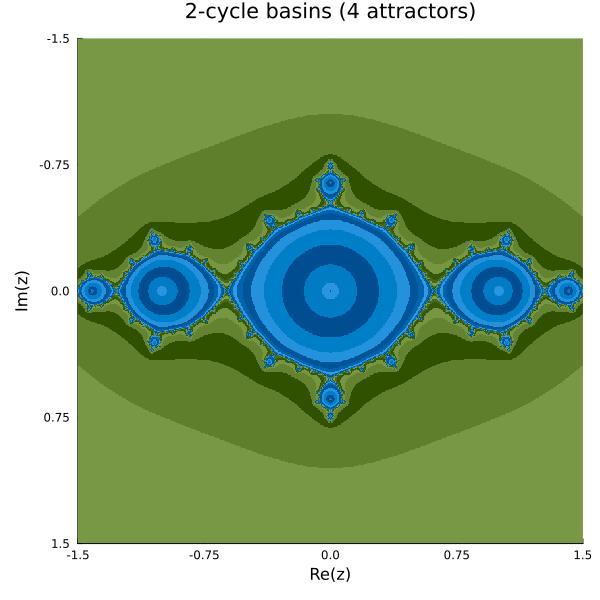
\includegraphics[width=0.55\textwidth]{figures/pcycle_z2.png}
  \caption{Cuencas del 2-ciclo $\{0,-1\}$ para $f(z)=z^2-1$,
           generadas con \fn{basin\_portrait\_pcycle}.
           Un único color cubre la cuenca completa del ciclo atractor;
           el negro corresponde a la cuenca del infinito.
           La frontera fractal refleja la simetría global de~$f$.}
  \label{fig:pcycle_z2}
\end{figure}

% ============================================================
\section{Ver las cuencas: una visualización matemáticamente fundada}
\label{sec:visualizacion}
% ============================================================

\subsection{El problema de la elección de colores}

La asignación de colores a las cuencas de atracción parece una decisión
estética, pero tiene implicaciones matemáticas y de comunicación
científica nada triviales.
Un conjunto de colores mal elegido puede hacer que dos cuencas parezcan
más similares de lo que son, o que la velocidad de convergencia sea
imposible de distinguir.
Más importante aún: un tercio de la población masculina presenta alguna
forma de daltonismo, y una visualización que dependa del rojo-verde —la
más habitual— resulta ilegible para esas personas.

\subsection{El espacio de color LCHab}

El espacio CIE $L^*a^*b^*$ (abreviado \emph{Lab}) fue diseñado por la
Comisión Internacional de Iluminación en 1976 para ser
\emph{perceptualmente uniforme}: diferencias iguales en las coordenadas
$L^*$, $a^*$, $b^*$ corresponden a diferencias aproximadamente iguales
en la percepción humana del color.

Su versión cilíndrica, el espacio \emph{LCHab}, usa:
\begin{itemize}
  \item $L^*\in[0,100]$: luminosidad ($L^*=0$ negro, $L^*=100$ blanco).
  \item $C^*\geq 0$: croma o saturación ($a^*=C^*\cos H^*$,\;
        $b^*=C^*\sin H^*$).
  \item $H^*\in[0^\circ,360^\circ)$: ángulo de tono.
\end{itemize}

Para asignar colores a $N$ cuencas de atracción, partimos de un color
semilla $(L_0^*, C_0^*, H_0^*)$ y distribuimos los tonos uniformemente:
\[
  H_k^* = H_0^* + k\,\frac{360^\circ}{N+1}, \qquad k=1,\ldots,N,
\]
manteniendo fijos $L_0^*$ y $C_0^*=\max(C_{\text{semilla}},40)$.
Al conservar la luminosidad y la croma, todos los colores resultantes
son perceptualmente equivalentes en brillo y saturación, independientemente
del ángulo de tono.
Esto garantiza que ninguna cuenca destaque artificialmente sobre las
demás por un efecto de contraste luminoso.

\begin{figure}[ht]
  \centering
  \begin{subfigure}[b]{0.47\textwidth}
    \centering
    % basin_portrait(num3, den3; bands=8.0, colorblind=false)
    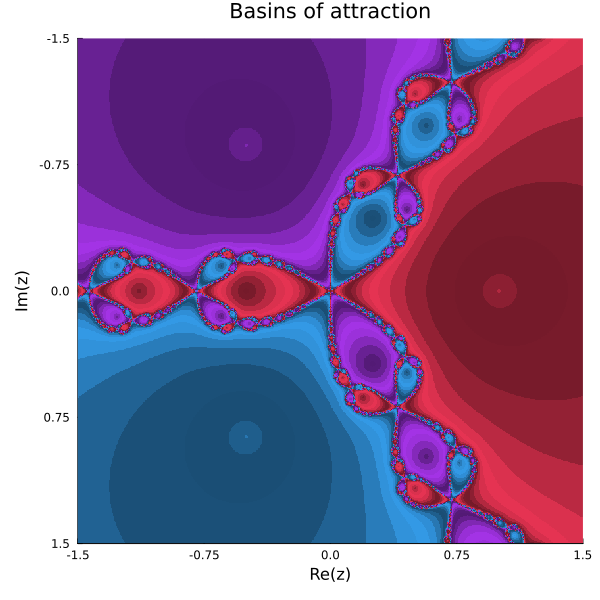
\includegraphics[width=\textwidth]{figures/newton_normal.png}
    \caption{Paleta LCHab estándar.}
  \end{subfigure}
  \hfill
  \begin{subfigure}[b]{0.47\textwidth}
    \centering
    % basin_portrait(num3, den3; bands=8.0, colorblind=true)
    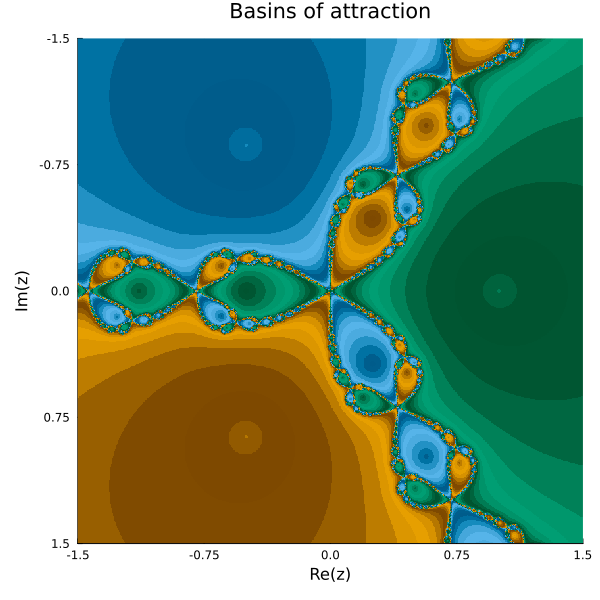
\includegraphics[width=\textwidth]{figures/newton_daltonico.png}
    \caption{Paleta Okabe--Ito (daltonismo).}
  \end{subfigure}
  \caption{Comparación de paletas para Newton en $z^3-1$.
           La paleta LCHab (izquierda) distribuye los tonos de forma
           equidistante en el espacio perceptual, maximizando el contraste
           entre cuencas para visión normal.
           La paleta Okabe--Ito~\cite{OkabeIto2008} (derecha) está
           diseñada para ser distinguible por personas con deuteranopía
           o protanopía, independientemente de los colores que aparezcan.
           Ambas conservan luminosidades equivalentes entre cuencas.}
  \label{fig:paletas}
\end{figure}

\subsection{Bandas de convergencia y conteo de iteraciones suavizado}

La velocidad con que una órbita se aproxima al atractor contiene
información geométrica rica.
Para visualizarla, usamos el \emph{conteo de iteraciones suavizado}.
Si la órbita de $z$ alcanza el atractor $\zeta$ tras $n$ iteraciones
con $|f^n(z)-\zeta|<\varepsilon$, definimos
\[
   \mu(z) = n - \frac{\log\log(|f^n(z)-\zeta|/\varepsilon)}{\log 2}
   \;\in\;\R_{\geq 0},
\]
que extiende el conteo entero a un valor real continuo y elimina la
discontinuidad que aparecería entre los niveles $n$ y $n+1$.
Modulamos entonces la luminosidad $L^*$ de cada píxel mediante:
\[
  L^*(z) = L_0^* + \Delta L\cdot\frac{1+\cos(2\pi\,b\,\tilde{\mu})}{2},
  \qquad \tilde{\mu}=\mu(z)/n_{\max},
\]
donde $b$ es el \emph{número de bandas} (parámetro del usuario) y
$\Delta L$ es la amplitud de la modulación.
El resultado son los anillos concéntricos visibles en la
figura~\ref{fig:bandas}: cada banda corresponde a una capa de puntos que tardan
aproximadamente el mismo número de iteraciones en converger.

\begin{figure}[ht]
  \centering
  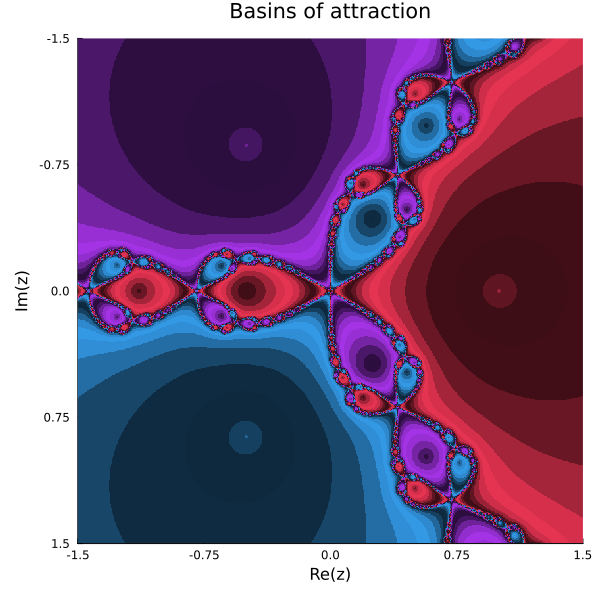
\includegraphics[width=0.60\textwidth]{figures/newton_bands.png}
  \caption{Efecto del bandeo en la visualización de Newton para $z^3-1$.
           La modulación de la luminosidad $L^*$ crea anillos concéntricos
           que revelan la velocidad de convergencia hacia cada atractor.
           Parámetro $b=8$ bandas.
           Generado con \pkg{RiemannBasins.jl}.}
  \label{fig:bandas}
\end{figure}

\subsection{El paquete \pkg{RiemannBasins.jl}}

Todas las figuras de este artículo han sido generadas con el paquete
\pkg{RiemannBasins.jl}~\cite{RiemannBasins2026}, escrito en Julia.
Las funciones racionales se especifican mediante listas de coeficientes
en coordenadas homogéneas, y la iteración se realiza directamente en
$\Puno$ para evitar los problemas de cancelación numérica cerca del
infinito.
Un ejemplo mínimo:

\begin{lstlisting}[caption={Retrato de cuencas para Newton en $z^3-1$ con visualización en las dos cartas de $\Puno$.}]
using RiemannBasins

# Numerador y denominador de N(z) = (2z^3+1)/(3z^2)
# Coeficientes en orden ascendente [a_0, a_1, ..., a_n]:
num = complex([1.0, 0.0, 0.0, 2.0])   # 1 + 2z^3 = 2z^3 + 1
den = complex([0.0, 0.0, 3.0, 0.0])   # 3z^2

# Retrato de cuencas en la carta estandar
basin_portrait(num, den; bands = 8.0)

# Retrato en las dos cartas estereograficas
two_chart_portrait(num, den; bands = 8.0)

# Superficie 3-D con GLMakie (requiere: using GLMakie)
basin_relief_3d_makie(num, den; bands = 50.0, relief_scale = 0.01)

# Cuencas de ciclos de periodo p (p = 2 en el ejemplo)
basin_portrait_pcycle(num, den, 2; bands = 8.0)
\end{lstlisting}

La superficie tridimensional (figura~\ref{fig:relief}) decouples color
y elevación: el color de cada elemento de superficie es el retrato LCHab
completo, mientras que la elevación codifica únicamente la geometría
de las fronteras fractales mediante el conteo de iteraciones suavizado.
Este desacoplamiento, posible gracias a la API de \pkg{GLMakie.jl}, no
es realizable con los motores de renderizado convencionales.

\begin{figure}[ht]
  \centering
  \begin{subfigure}[t]{0.47\textwidth}
    % Comando: basin_relief_3d_makie(num, den; bands=8.0, relief_scale=0.001,
    %          savepath="figures/relief_low.png")
    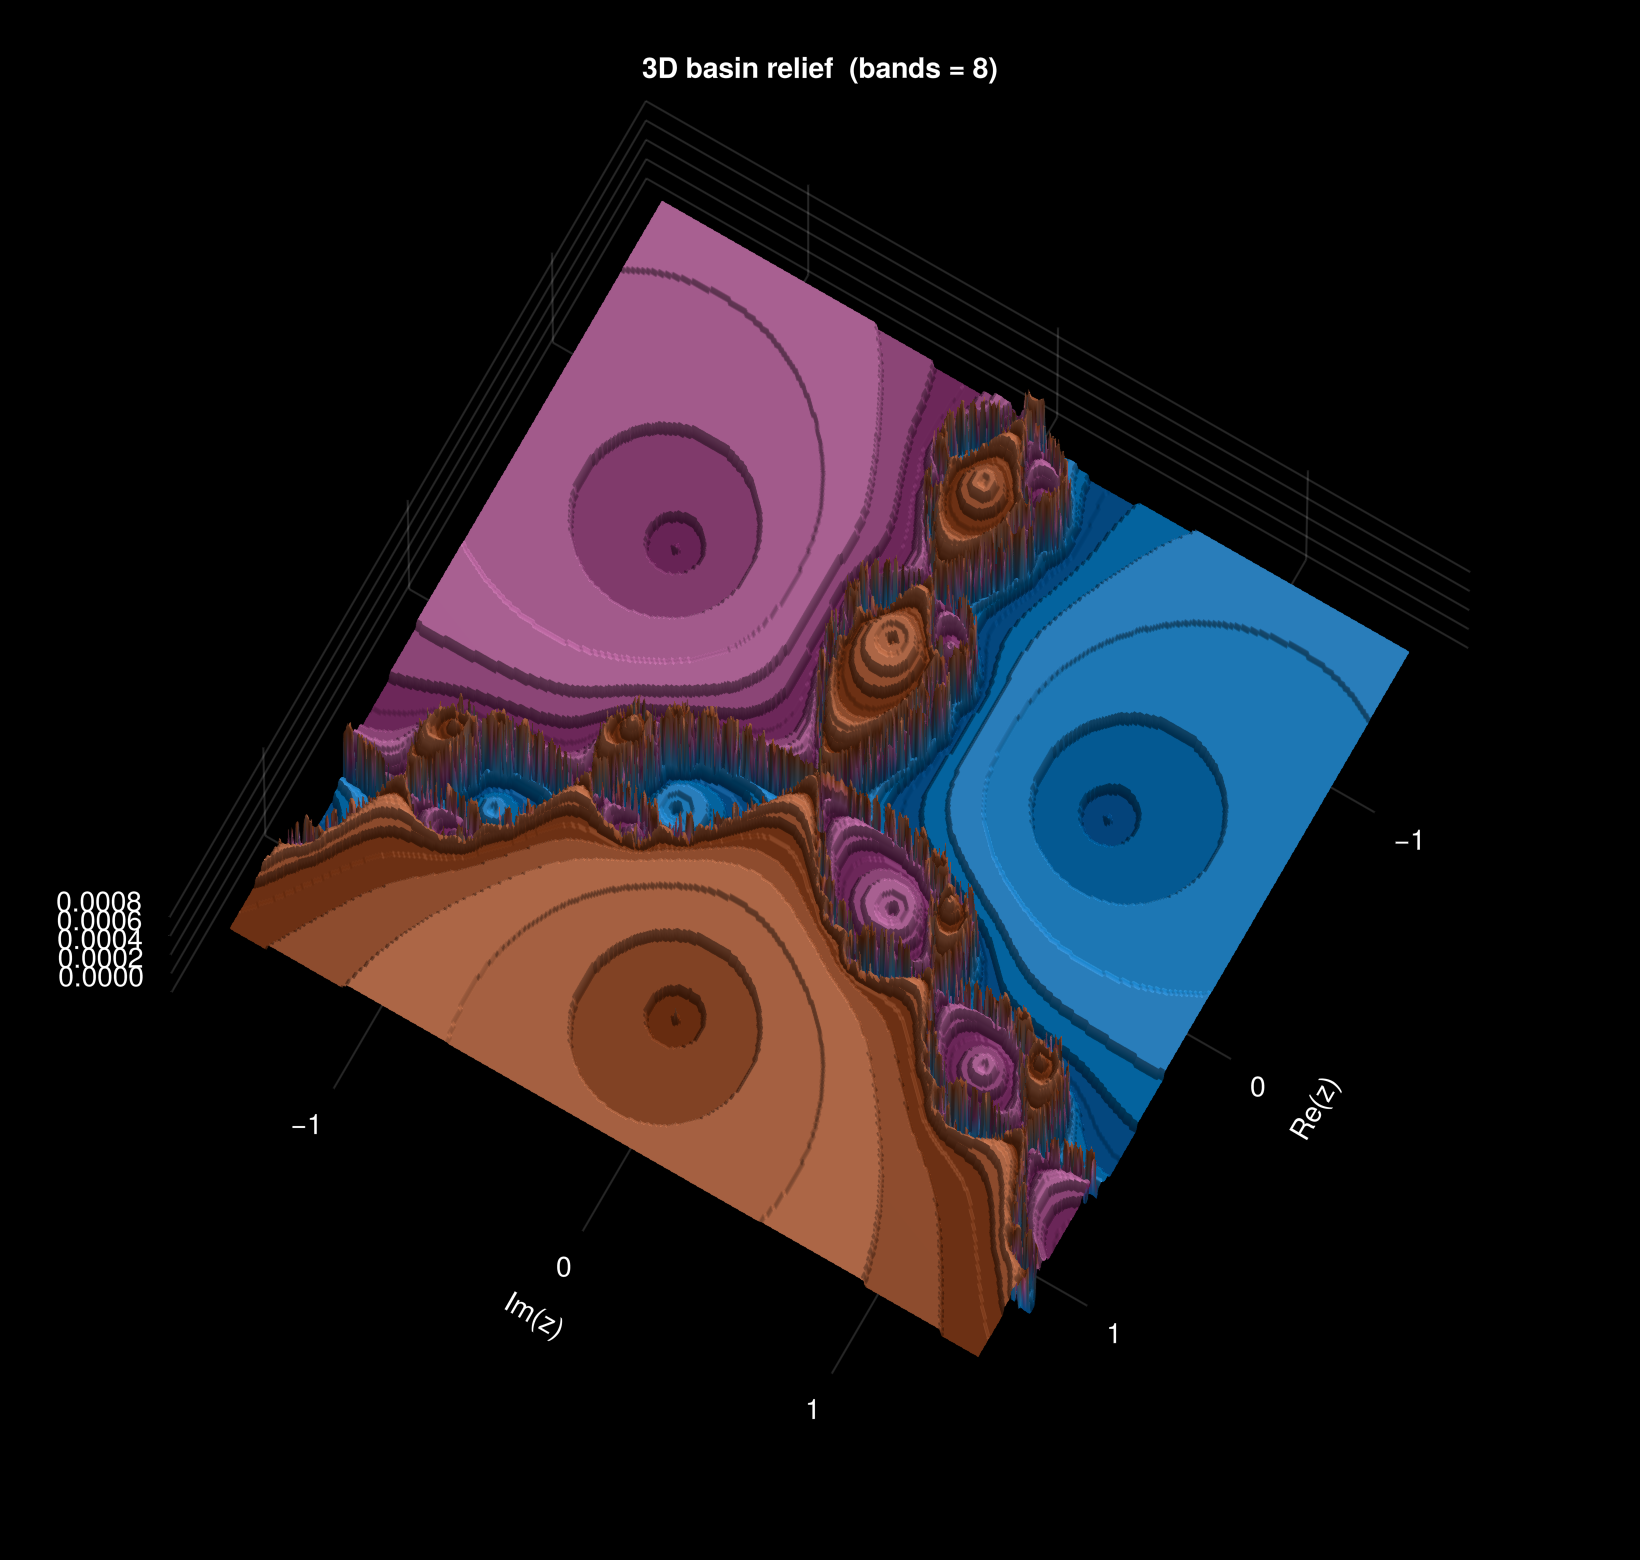
\includegraphics[width=\textwidth]{figures/relief_low.png}
    \caption{Relieve bajo (\texttt{relief\_scale=0.001}):
             la información de color domina; el conjunto de Julia
             aparece como una textura cromática.}
  \end{subfigure}\hfill
  \begin{subfigure}[t]{0.47\textwidth}
    % Comando: basin_relief_3d_makie(num, den; bands=8.0, relief_scale=0.05,
    %          savepath="figures/relief_high.png")
    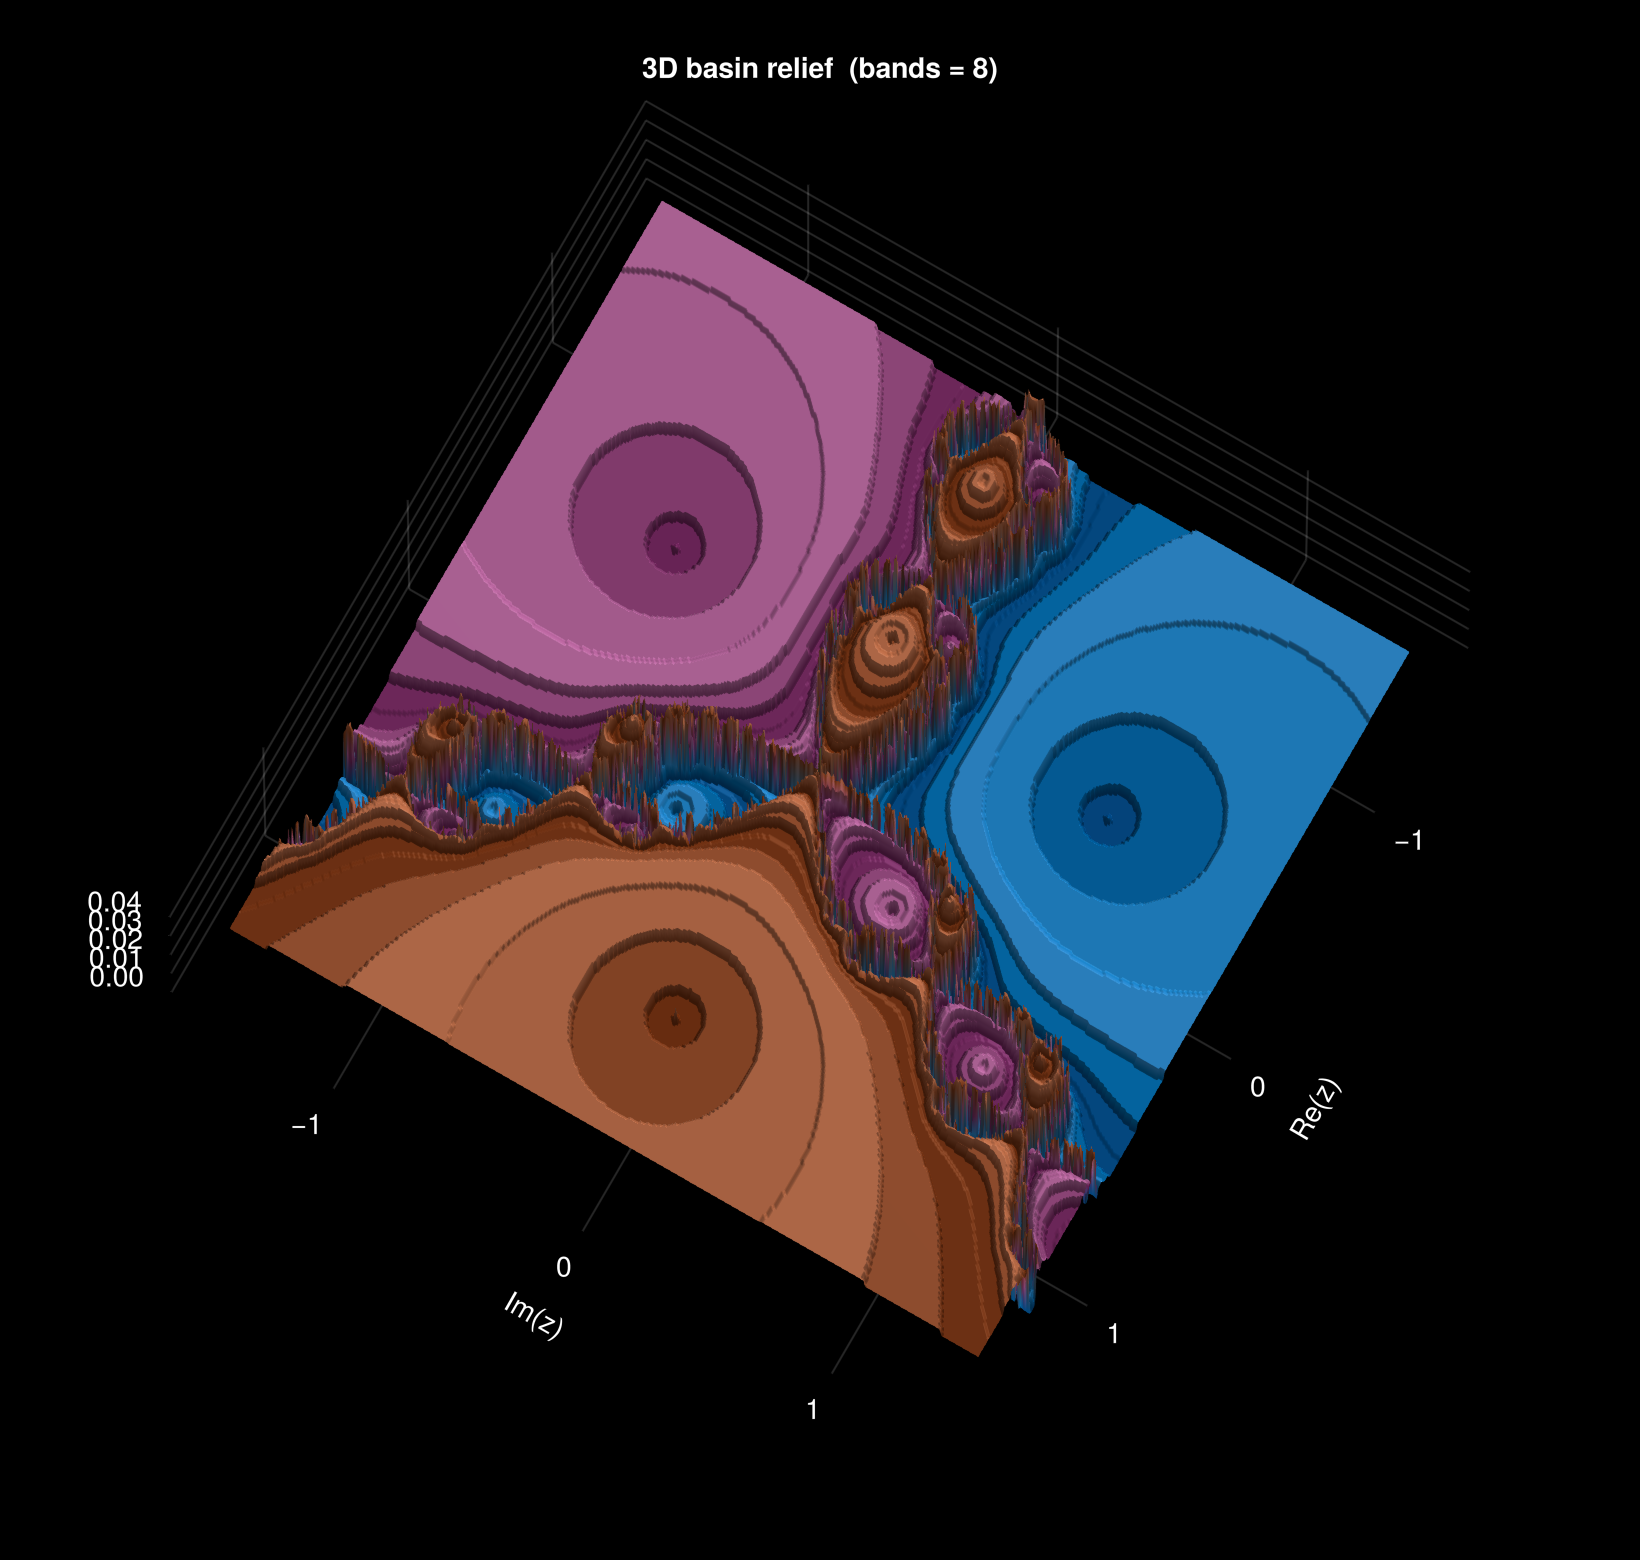
\includegraphics[width=\textwidth]{figures/relief_high.png}
    \caption{Relieve alto (\texttt{relief\_scale=0.05}):
             la topografía fractal del conjunto de Julia emerge
             como una sierra tridimensional.}
  \end{subfigure}
  \caption{Efecto del parámetro \texttt{relief\_scale} en la superficie
           tridimensional para Newton en $z^3-1$, generada con
           \pkg{GLMakie.jl}.
           Color y elevación son independientes: el color refleja el
           retrato de cuencas LCHab; la elevación, el conteo de
           iteraciones suavizado en la frontera fractal.}
  \label{fig:relief}
\end{figure}

% ============================================================
\section{Conclusión y perspectivas}
\label{sec:conclusion}
% ============================================================

Hemos mostrado que el espacio proyectivo $\Puno$ es el dominio natural
para la dinámica de iteración de funciones racionales.
Trabajar en coordenadas homogéneas, en lugar de en $\C$ con el infinito
tratado como caso especial, tiene consecuencias concretas: el
Teorema~\ref{teo:puntosfijos} da exactamente $d+1$ puntos fijos, la
segunda carta estereográfica hace visible la cuenca del infinito, y la
simetría global del sistema queda de manifiesto.

Los ejemplos de Milnor —Newton, Halley, la familia $z^2+c$— ilustran
que distintas estrategias de iteración producen estructuras globalmente
distintas en~$\Puno$, y que la geometría de las cuencas en la segunda
carta completa el cuadro que la carta afín estándar deja parcialmente
oculto.

La elección de colores en el espacio LCHab garantiza visualizaciones
perceptualmente honestas: todas las cuencas son igualmente visibles,
la velocidad de convergencia se codifica en una señal visual continua,
y las paletas para daltonismo permiten que el material sea accesible
para toda la audiencia.

El paquete incluye ya la detección de ciclos atractores de período
$p\geq 2$ mediante la función \fn{basin\_portrait\_pcycle}
(subsección~\ref{ssec:pcycle_z2}): dado un entero $p\geq 1$, la
función compone $f^p$ simbólicamente, agrupa sus puntos fijos por
órbita bajo $f$, e itera $f^p$ píxel a píxel para colorear las cuencas.
Esto permite visualizar la dinámica completa de familias como $z^2+c$,
donde el período del ciclo atractor varía con~$c$.

Quedan abiertas otras líneas de trabajo, de distinto grado de
especulación.

La primera concierne la dinámica de \emph{pares} de funciones
racionales.
Si $\mathbb{Z}$ denota el grupo cíclico infinito, cada función
racional $f$ de transformación de Möbius genera una acción de
$\mathbb{Z}$ en $\Puno$ mediante la iteración $n\mapsto f^n$.
Dadas dos transformaciones $f$ y $g$, el grupo que generan es en
general el producto libre $\mathbb{Z}\star\mathbb{Z}$,
cuya acción en~$\Puno$ da lugar a un \emph{grupo de Kleinian}.
El conjunto de Fatou del grupo es la región maximal donde toda
sucesión de composiciones de $f^{\pm 1}$ y $g^{\pm 1}$ forma una
familia normal; su complementario es el conjunto de Julia del grupo.
Para funciones racionales de grado $\geq 2$ (no invertibles) el
objeto análogo es el \emph{semigrupo racional} $\langle f,g\rangle$,
cuya teoría de Fatou-Julia fue iniciada por Hinkkanen y Martin.
Visualizar las cuencas de atracción de $\mathbb{Z}\star\mathbb{Z}$
en~$\Puno$ permitiría comparar métodos numéricos —Newton, Halley,
secantes— dentro de un marco algebraico unificado.

La segunda línea, más inmediata, es la extensión de
\fn{basin\_portrait\_pcycle} a la detección automática del período
mínimo del ciclo atractor, evitando calcular $f^p$ para valores de~$p$
que el usuario ha de especificar a priori.

% ============================================================
\section*{Agradecimientos}
% ============================================================

El paquete \pkg{RiemannBasins.jl} fue desarrollado con asistencia del
modelo de lenguaje Claude (Anthropic).
El autor agradece igualmente su contribución en la discusión de los
enfoques y la estructuración del presente artículo.

% ============================================================
\begin{thebibliography}{9}
% ============================================================

\bibitem{HinkkanenMartin1996}
A.~Hinkkanen e~I.~N.~Martin,
«The dynamics of semigroups of rational functions I»,
\textit{Proc.\ London Math.\ Soc.} \textbf{73} (1996), 358--384.

\bibitem{Milnor2006}
J.~Milnor,
\textit{Dynamics in One Complex Variable},
3.ª~ed., Princeton University Press, Princeton, 2006.

\bibitem{Beardon1991}
A.~F.~Beardon,
\textit{Iteration of Rational Functions},
Springer-Verlag, Nueva York, 1991.

\bibitem{CarlsonEtAl1994}
N.~Carlson, D.~Mandell y J.~F.~Epperson,
«Newton's method for the complex cube roots of unity»,
\textit{Amer.\ Math.\ Monthly} \textbf{101} (1994), 645--648.

\bibitem{OkabeIto2008}
M.~Okabe e~I.~Ito,
«Color universal design (CUD): how to make figures and presentations
that are friendly to colorblind people»,
\textit{J.\ Jap.\ Assoc.\ Human Genetics} \textbf{53} (2008), 1--7.

\bibitem{Fairchild2013}
M.~D.~Fairchild,
\textit{Color Appearance Models},
3.ª~ed., Wiley, 2013.

\bibitem{RiemannBasins2026}
L.~J.~Hernández~Paricio,
\textit{RiemannBasins.jl: visualización de cuencas de atracción de
funciones racionales en la esfera de Riemann},
Universidad de La Rioja, 2026.
Disponible en: \url{https://github.com/luhernan/RiemannBasins.jl}

\end{thebibliography}

\end{document}
